\documentclass[11pt]{article}
\usepackage[left=2.5cm,right=2.5cm,top=2.5cm,bottom=2.5cm]{geometry}
\usepackage[T1]{fontenc}
\usepackage[utf8]{inputenc}
\usepackage{lmodern}
\usepackage{amsmath}
\usepackage{siunitx}
\usepackage{booktabs}
\usepackage{tabularx}
\usepackage{array}
\usepackage{xcolor}
\usepackage{tikz}
\usepackage[hidelinks]{hyperref}
\usetikzlibrary{arrows.meta, positioning, calc}

\setlength{\parindent}{0mm}
\setlength{\parskip}{2mm}
\renewcommand{\arraystretch}{1.25}
\newcolumntype{L}{>{\raggedright\arraybackslash}X}

% Marks a value that is assumed and must be confirmed
\newcommand{\assumed}{\textsuperscript{\textcolor{red}{A}}}

% Generated from CasRioSim/design_basis.toml by CasRioSim/tools/design_report.py
% GENERATED by CasDesignBasis/tools/design_report.py from design_basis.toml v2.2.0. Do not edit.
\newcommand{\CASVersion}{2.2.0}
\newcommand{\CASNomMode}{O-45}
\newcommand{\CASNomPumps}{2}
\newcommand{\CASTs}{1}
\newcommand{\CASGainLevel}{1.339}
\newcommand{\CASGainOxy}{0.1067}
\newcommand{\CASGainR}{-0.1333}
\newcommand{\CASGainN}{-0.0104}


\title{CAS (Heimdall) -- design basis for control\\[1mm]
\large Parameters, dynamic model and linear model\\[1mm]
\normalsize Design basis version \CASVersion}
\author{Sigurd R. Brekk}
\date{\today}

\begin{document}
\maketitle

\section{Purpose}

This document sets out the parameters and the dynamic model used to design the level and oxygen
control for the ScaleAQ closed aquaculture system (CAS), PLC project Heimdall. Every parameter
has a value, a unit, a source and a reason for the choice. It replaces the parameter set in
\emph{CAS model.tex}; Section~\ref{tab:changes} lists the changes.

\textbf{One source of truth.} The parameters live in \texttt{design\_basis.toml} [TOML] and the
equations in \texttt{casriosim/design.py} [MODEL], both in \texttt{workfolder-python/CasRioSim}.
The simulator CasRioSim integrates exactly these equations, and its version is the design basis
version (\CASVersion). The tables, matrices and difference equations in this document are
generated from the same files by \texttt{tools/design\_report.py} [PY] into
\texttt{generated/}. To change the design:
\begin{enumerate}
  \item change \texttt{design\_basis.toml} (or \texttt{design.py}) and bump
        \texttt{meta.version};
  \item run \texttt{python tools/selftest\_model.py}, which checks that the simulator's model
        linearizes to exactly the matrices in Section~\ref{sec:linear};
  \item run \texttt{python tools/design\_report.py} and rebuild this document;
  \item push to \texttt{main}. CI publishes the simulator image with the new version.
\end{enumerate}

Values marked \assumed{} are assumptions that are not yet supported by a document. They are
listed in Section~\ref{sec:open} and must be confirmed.

\subsection*{Sources}
\begin{tabularx}{\textwidth}{@{}lL@{}}
\toprule
ID & Document \\
\midrule
{[DB]}    & 10925-CAS-001-02 Design basis, rev.~2, Automation (working document) \\
{[FD]}    & P-15169-CAS-FD-01 Funksjonsbeskrivelse CAS, rev.~B incl.\ tracked changes up to 28.09.26 \\
{[SPEC]}  & Framo 0000\_CAS\_SPEC\_CTRLSYS, Kontrollsystem (prototype), rev.~B, 08.10.2025 \\
{[SR2000]}& Framo SR2000 pump specification (datasheet) \\
{[PF]}    & pumpeflow\_Sr2000\_CAS.xlsx (pump power and system head reference) \\
{[O2S]}   & Beregningsark dimensjonering ved bortfall av pumper eller strøm, 17.03.26 \\
{[CT]}    & Oppsett innløsere CT.xlsx (Chucaotech oxygenator sizing) \\
{[CTE]}   & CT002-CS-022 v0-2, oxygen transfer efficiency test, 23.07.2024 \\
{[B2865]} & Bürkert 2865 proportional valve, datasheet \\
{[S418]}  & SUTO S418 flow meter, datasheet \\
{[RDO]}   & RDO Core (Orbit 864) dissolved oxygen sensor, spec sheet \\
{[VEGA]}  & VEGAPULS C 21 radar level sensor, specification sheet \\
{[LTU]}   & LTU801 pressure level transmitter, IOM \\
{[SO]}    & Sensor Overview CAS V1.xlsx \\
{[B8605]} & Bürkert 8605 PWM driver, Linde default setup, 22.02.22 \\
{[W455]}  & WAGO 750-455 4AI 4--20\,mA product manual, 2453453963, valid from HW 07 / FW 04 \\
{[TOML]}  & CasRioSim/design\_basis.toml, version \CASVersion{} (all parameters) \\
{[MODEL]} & CasRioSim/casriosim/design.py (model equations, used by the simulator) \\
{[PY]}    & CasRioSim/tools/design\_report.py (generates this document's tables) \\
\bottomrule
\end{tabularx}

\section{System and control structure}

Water is pumped into the pen by three Framo SR2000 inlet pumps through flexible tunnels taken in
at 10--30\,m depth. It leaves through a bottom centre outlet that has four hydraulic dampers. The
pen level is held a few centimetres above the outside sea level (the \emph{over-height}
$\Delta h$), and that over-height drives the outflow. Oxygen is dissolved in a side stream on
each inlet (oxy-pump and Chucaotech oxygenator), with one oxygen gas flow loop per line.

The control structure follows [FD] §3.2.2--3.2.4 (Figure~\ref{fig:structure}):
\begin{itemize}
  \item \textbf{LIC01}, level: PI on $\Delta h_\text{avg}$. It sends one common speed setpoint
        to all running inlet pumps. The dampers are held at a fixed opening per operating mode.
  \item \textbf{OIC01}, oxygen (master): PI on one pen O$_2$ sensor, normally OT03 at the outlet.
        Its output is the setpoint for the three O$_2$ flow loops.
  \item \textbf{FIC41--43}, O$_2$ flow (slave): PI on the gas flow (FT41--43). It drives the
        PWM proportional valve OV41--43.
\end{itemize}

\begin{figure}[h]
\centering
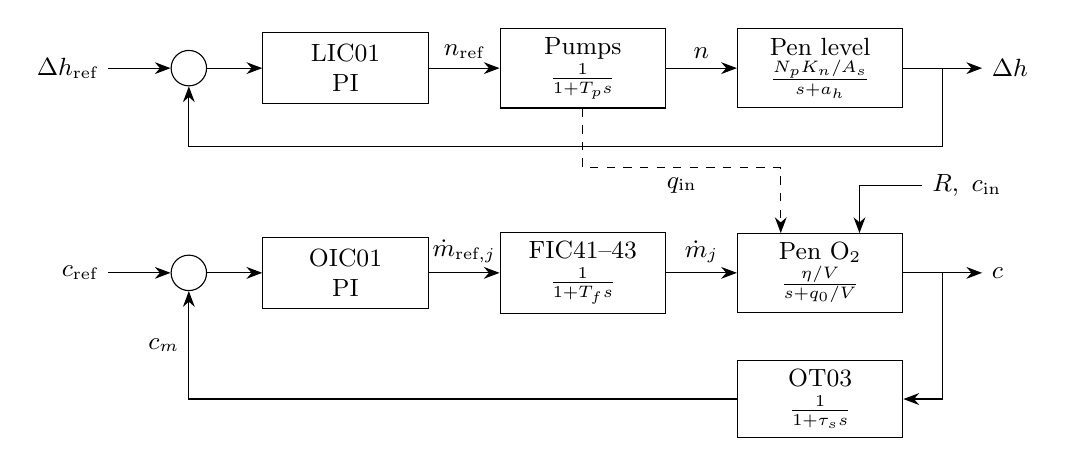
\begin{tikzpicture}[
  blk/.style={draw, minimum width=2.1cm, minimum height=0.9cm, align=center, font=\small},
  sum/.style={draw, circle, minimum size=0.45cm, inner sep=0},
  >={Stealth[length=2mm]}, font=\small]
  % level loop
  \node[sum] (s1) at (0,0) {};
  \node[blk, right=0.7cm of s1] (lic) {LIC01\\PI};
  \node[blk, right=0.9cm of lic] (pump) {Pumps\\$\frac{1}{1+T_ps}$};
  \node[blk, right=0.9cm of pump] (lev) {Pen level\\$\frac{N_pK_n/A_s}{s+a_h}$};
  \draw[<-] (s1.west) -- ++(-0.8,0) node[left] {$\Delta h_\text{ref}$};
  \draw[->] (s1) -- (lic);
  \draw[->] (lic) -- node[above] {$n_\text{ref}$} (pump);
  \draw[->] (pump) -- node[above] {$n$} (lev);
  \draw[->] (lev.east) -- ++(1.0,0) node[right] {$\Delta h$};
  \draw[->] ($(lev.east)+(0.5,0)$) -- ++(0,-1.0) -| (s1.south);
  % oxygen loop
  \node[sum] (s2) at (0,-2.6) {};
  \node[blk, right=0.7cm of s2] (oic) {OIC01\\PI};
  \node[blk, right=0.9cm of oic] (fic) {FIC41--43\\$\frac{1}{1+T_fs}$};
  \node[blk, right=0.9cm of fic] (pen) {Pen O$_2$\\$\frac{\eta/V}{s+q_0/V}$};
  \node[blk, below=0.6cm of pen] (sens) {OT03\\$\frac{1}{1+\tau_ss}$};
  \draw[<-] (s2.west) -- ++(-0.8,0) node[left] {$c_\text{ref}$};
  \draw[->] (s2) -- (oic);
  \draw[->] (oic) -- node[above] {$\dot m_{\text{ref},j}$} (fic);
  \draw[->] (fic) -- node[above] {$\dot m_j$} (pen);
  \draw[->] (pen.east) -- ++(1.0,0) node[right] {$c$};
  \draw[->] ($(pen.east)+(0.5,0)$) |- (sens.east);
  \draw[->] (sens.west) -| node[near end, left] {$c_m$} (s2.south);
  % coupling
  \draw[->, dashed] (pump.south) -- ++(0,-0.75) -| node[pos=0.25, below] {$q_\text{in}$} ($(pen.north)+(-0.5,0)$);
  \draw[<-] ($(pen.north)+(0.5,0)$) -- ++(0,0.6) -- ++(0.8,0) node[right] {$R,\ c_\text{in}$};
\end{tikzpicture}
\caption{Control structure. The dashed line is the coupling from pump flow to oxygen.}
\label{fig:structure}
\end{figure}

\section{Parameters}

All tables in this section are generated from [TOML]; each row carries its own source and
reason there.

\subsection{Pen and outlet}
% GENERATED by CasDesignBasis/tools/design_report.py from design_basis.toml v2.3.1. Do not edit.
\begin{tabularx}{\textwidth}{@{}l r l l L@{}}
\toprule
Symbol & Value & Unit & Source & Reason \\
\midrule
$V$ & \num{20000} & m$^3$ & [DB] 1.2 & Design volume. \\
$D$ & \num{50.5} & m & [DB] tab. 7 & Tarpaulin diameter. The free surface $A_s = \pi D^2/4$ sets the level capacitance; the surface is treated as rigid. \\
$D_o$ & \num{17.3} & m & [DB] tab. 7 & Tarpaulin depth, taken as the outlet depth. \\
$\rho$ & \num{1025} & kg/m$^3$ & [DB] tab. 21 & Sea water density. \\
$\Delta\rho$ & \num{2} & kg/m$^3$ & [DB] 4.4.1 & Density difference [DB] uses for the inner water height. Inside water from 10--30 m is assumed denser, giving the extra outlet head $h_\rho = D_o\Delta\rho/\rho$.\assumed{} \\
$\text{full-open mode}$ & O-45 & -- & [FD] tab. 10, [DB] tab. 16 & Outlet conductance at full damper opening, taken from O-45. O-35 and O-45 give the same conductance (30.8 vs. 30.9), consistent with a fully open outlet. Conductance is assumed linear in the opening.\assumed{} \\
$A_s$ & 2003 & m$^2$ & $\pi D^2/4$ & Free surface area. \\
$h_\rho$ & 3.38 & cm & $D_o\Delta\rho/\rho$ & Extra driving head at the outlet. \\
$k_{d,\text{full}}$ & 30.94 & m$^{2.5}$/s & $Q_0/\sqrt{\Delta h_0+h_\rho}$ & Outlet conductance at full opening (O-45). \\
\bottomrule
\end{tabularx}


\subsection{Inlet pumps}
% GENERATED by CasDesignBasis/tools/design_report.py from design_basis.toml v2.3.2. Do not edit.
\begin{tabularx}{\textwidth}{@{}l r l l L@{}}
\toprule
Symbol & Value & Unit & Source & Reason \\
\midrule
$Q_\text{rated}$ & \num{20000} & m$^3$/h & [SR2000] & Rated flow at rated speed. \\
$n_\text{min}$ & \num{40} & rpm & [SR2000], [FD] tab. 8 & Minimum speed, also the LIC01 output range. \\
$n_\text{max}$ & \num{130} & rpm & [SR2000], [FD] tab. 8 & Maximum speed. $K_n = Q_\text{rated}/n_\text{max}$ by the affinity law $Q\propto n$, which holds because the system head is almost purely $\propto Q^2$ [PF] and the static over-height is below 10 cm. \\
$N$ & \num{3} & -- & [DB] 3.4 & Three inlets, each with one SR2000 and one oxygenator. \\
$T_p$ & \num{10} & s & - & Time constant from speed setpoint to actual speed (VSD ramp and water column). To be confirmed by Framo.\assumed{} \\
$P_\text{max}$ & \num{60} & kW & [SR2000] & Motor power at $n_\text{max}$. Power follows the affinity law $P = P_\text{max}(n/n_\text{max})^3$; at 130 rpm this gives the datasheet torque of 4407 Nm. \\
$z_p$ & \num{72} & -- & [SR2000] & Motor poles. Electrical frequency $f = n z_p/120$, 78 Hz at 130 rpm. \\
$I_\text{rated}$ & \num{110} & A & [SR2000] & Rated current at 400 V. Current is scaled from power and voltage. \\
$U_\text{rated}$ & \num{400} & V & [SR2000] & Rated voltage. Motor voltage is taken proportional to frequency (V/f). \\
$K_n$ & 0.042735 & (m$^3$/s)/rpm & $Q_\text{rated}/n_\text{max}$ & Flow per rpm. \\
\bottomrule
\end{tabularx}


\subsection{Operating modes}
Flow, level setpoint and number of pumps per mode come from [FD] tab.~10 and [DB] tab.~16. The
other columns follow from the model: $n_0 = Q_0/(N_pK_n)$, $k_d = Q_0/\sqrt{\Delta h_0+h_\rho}$,
the damper opening $k_d/k_{d,\text{full}}$, and the level time constant $1/a_h$
(Section~\ref{sec:linear}).

\begin{center}
% GENERATED by CasDesignBasis/tools/design_report.py from design_basis.toml v2.3.1. Do not edit.
\begin{tabular}{@{}l r r c r r r r@{}}
\toprule
Mode & $Q_0$ [m$^3$/h] & $\Delta h_0$ [cm] & $N_p$ & $n_0$ [rpm] & $k_d$ [m$^{2.5}$/s] & Opening [\%] & $1/a_h$ [s] \\
\midrule
O-35 & \num{34000} & 6.0 & 3 & 73.7 & 30.84 & 100 & 39.8 \\
O-45 & \num{27000} & 2.5 & 2 & 87.8 & 30.94 & 100 & 31.4 \\
O-60 & \num{20000} & 0.5 & 2 & 65.0 & 28.22 & 91 & 27.9 \\
S-75 & \num{16000} & 0.5 & 2 & 52.0 & 22.58 & 73 & 34.9 \\
\bottomrule
\end{tabular}

\end{center}

\textbf{\CASNomMode{} is the nominal design point.} It is the [DB] dimensioning case (case~3:
1\,000\,t, 27\,000\,m$^3$/h, 45\,min), and the mode that must be held with one pump out. The
linear model and the discrete equations are given for \CASNomMode{} with \CASNomPumps{} pumps.

\subsection{Water and oxygen}
% GENERATED by CasRioSim/tools/design_report.py from design_basis.toml v2.0.0. Do not edit.
\begin{tabularx}{\textwidth}{@{}l r l l L@{}}
\toprule
Symbol & Value & Unit & Source & Reason \\
\midrule
$T_w$ & \num{10} & °C & [DB] tab. 21 & Design temperature. \\
$S_w$ & \num{34} & ppt & [O2S] & Salinity. \\
$c_\text{in}/c_\text{sat}$ & \num{0.8} & -- & [O2S] & Intake water at 80 \% O$_2$ saturation; saturation by the Weiss formula of [O2S]. \\
$c_\text{ref}/c_\text{sat}$ & \num{0.9} & -- & [O2S] & Outlet design criterion, 90 \% saturation. [FD] has no O$_2$ setpoint yet.\assumed{} \\
\bottomrule
\end{tabularx}


% GENERATED by CasDesignBasis/tools/design_report.py from design_basis.toml v2.3.2. Do not edit.
\begin{tabularx}{\textwidth}{@{}l r l l L@{}}
\toprule
Symbol & Value & Unit & Source & Reason \\
\midrule
$\dot m_\text{max}$ & \num{104.2} & kg/h & [DB] tab. 13, [CT] & Maximum O$_2$ gas flow per oxygenator (CT10, sea water, 15 \% gas/liquid ratio). An oxygenator adds O$_2$ only while its own inlet pump runs. \\
$\eta$ & \num{0.8} & -- & [CTE] & Transfer efficiency; the test gave 0.81 initial efficiency, rounded down.\assumed{} \\
$T_f$ & \num{2} & s & design choice & Closed-loop time constant of FIC41-43, used in the control design model. \\
$\tau_v$ & \num{0.22} & s & [B2865], [S418] & Open-loop lag of valve and flow meter, used in the simulator: valve $<25$ ms, flow meter $t_{90}=0.5$ s ($\tau_v = t_{90}/\ln 10$). \\
$u_\text{cut}$ & \num{2} & \% & [B8605] & Driver cut-off; below this the valve is closed (Linde default). Above it the gas flow is linear in the command up to $\dot m_\text{max}$. \\
$u_\%$ & 4-20 mA & -- & user, [B8605] & 4 mA (0 \%) = fully closed, 20 mA (100 \%) = fully open. The PLC writes 0--32760 for 0--100 \% to the 750-563 output; the Bürkert 8605 driver takes the 4--20 mA (Linde default) and sets the coil current. Below the cut-off the valve stays closed, so a lost signal is expected to close the valve (no O$_2$ on that line). \\
$\tau_s$ & \num{19.54} & s & [RDO] & O$_2$ sensor as first order fitted to $T_{90}<45$ s ($\tau_s=T_{90}/\ln 10$). [RDO] gives $T_{63}<5$ s, so this is conservative. \\
$c_\text{sat}$ & 9.09 & g/m$^3$ & [O2S] & Saturation at $T_w$, $S_w$ (Weiss). \\
$c_\text{in}$ & 7.27 & g/m$^3$ &  & O$_2$ in the intake water. \\
$c_\text{ref}$ & 8.18 & g/m$^3$ &  & O$_2$ setpoint. \\
$\dot m_\text{max}$ & 28.94 & g/s &  & Maximum O$_2$ gas flow per line. \\
\bottomrule
\end{tabularx}


$T_f$ is used in the control design model, where FIC41--43 is closed. $\tau_v$ and the cut-off
are used in the simulator, where the PLC's FIC drives the valve itself
(Section~\ref{sec:sim}).

\subsection{Fish}
% GENERATED by CasDesignBasis/tools/design_report.py from design_basis.toml v2.3.1. Do not edit.
\begin{tabularx}{\textwidth}{@{}l r l l L@{}}
\toprule
Symbol & Value & Unit & Source & Reason \\
\midrule
$\rho_f$ & \num{50} & kg/m$^3$ & [DB] 1.2 & Maximum density; biomass $B = \rho_f V$. \\
$W$ & \num{1000} & g & [DB] tab. 18 & Average weight, [DB] case 3. \\
$U$ & \num{41} & cm/s & [O2S] & Recommended swimming speed for 1 kg at 10 °C. \\
$B$ & \num{1000000} & kg & $\rho_f V$ & Maximum biomass. \\
$r$ & 3.26 & mg/(kg\,min) & [O2S] & Average post-smolt salmon, $r = 1.92\,W^{-0.27}T^{0.63}10^{0.01U}$ ($=196$\,mg/(kg\,h)). \\
$R_0$ & 54.3 & g/s & $rB$ & Nominal total O$_2$ consumption of the fish. \\
\bottomrule
\end{tabularx}


\subsection{Level measurement}
% GENERATED by CasDesignBasis/tools/design_report.py from design_basis.toml v2.3.1. Do not edit.
\begin{tabularx}{\textwidth}{@{}l r l l L@{}}
\toprule
Symbol & Value & Unit & Source & Reason \\
\midrule
$\text{LT01--03}$ & \num{2} & mm & [VEGA], [SO] & Radar, deviation $\leq 2$ mm. \\
$\text{LT21--23}$ & \num{4} & mm & [LTU], [SO] & Pressure transmitter, 0.2 \% of an assumed 2 m full scale.\assumed{} \\
$h_\text{span}$ & \num{2} & m & [VEGA], [W455], user & Span of the 4--20 mA level signal. The 750-455 resolves it with 12 bits: 0--4095 in bits 14--3 of the word (20 mA = 0x7FF8, status in bits 2--0), so one step is $2000/4095 = 0.49$ mm, inside the $\pm 2$ mm sensor deviation. The HW 07 manual [W455] instead places 20 mA at 0x7FF0 (bits 15--4, 0.98 mm steps); the installed hardware decides which. \\
$\text{raw } 0$ & low & -- & [VEGA] & Which end of the span reads 0 (4 mA). "low": 0 = lowest water level in the span (VEGA level-proportional output, 4 mA = min. adjustment). "high": 0 = highest level, as when the output follows the measured distance from the antenna. Not stated in the datasheets; read the min./max. adjustment and current output mode in the sensor.\assumed{} \\
$h_\text{out,0}$ & \num{1} & m & - & Outside sea level within the span, mid-range. Set by the sensor mounting height.\assumed{} \\
$\text{OT01--03, OT21--22}$ & \num{5} & -- & [RDOM], [W652], [HEIM] & In-Situ RDO Core (Orbit 864), Modbus RTU on the RS-485 line of the 750-652, the first module on CommonRIO (Modbus words 0--11). Three inside the pen (slave addresses 1--3), two outside (4--5), as in Heimdall (GVL\_CONSTANT); the cabinet drawing shows six. 9600 baud 8N1, as ScaleAQ configures them (Assembly Manual DOC100486-04). Idle sensors sleep and answer the waking request late; Heimdall retries, or writes Communication Stay Awake (register 9210). The inside sensors read $c_m$, the outside ones $c_\text{in}$. DO in mg/L as a float at registers 40038--39. \\
$z_\text{OT}$ & \num{3} & m & - & Sensor depth, for the simulated pressure reading. Not in the design documents.\assumed{} \\
\bottomrule
\end{tabularx}


The PV range of LIC01 is 0--20\,cm [FD] tab.~8, the mean over the active sensor pairs.

\section{Dynamic model}\label{sec:model}

\subsection{States, inputs and disturbances}
\begin{align*}
x_1 &= \Delta h \ \text{[m], over-height}                     & u_1 &= n_\text{ref}\ \text{[rpm], common pump speed setpoint}\\
x_2 &= n \ \text{[rpm], actual pump speed}                     & u_2 &= \dot m_{\text{ref},1}\ \text{[g/s], O$_2$ flow setpoint line 1}\\
x_3 &= c \ \text{[g/m$^3$], O$_2$ concentration in pen}         & u_3 &= \dot m_{\text{ref},2}\ \text{[g/s], line 2}\\
x_4 &= \dot m_1 \ \text{[g/s], O$_2$ gas flow line 1}           & u_4 &= \dot m_{\text{ref},3}\ \text{[g/s], line 3}\\
x_5 &= \dot m_2 \ \text{[g/s], line 2}                          & d_1 &= R\ \text{[g/s], O$_2$ consumption of fish}\\
x_6 &= \dot m_3 \ \text{[g/s], line 3}                          & d_2 &= c_\text{in}\ \text{[g/m$^3$], O$_2$ in intake water}\\
x_7 &= c_m \ \text{[g/m$^3$], measured O$_2$ (OT03)}            &     &
\end{align*}

The O$_2$ inputs are setpoints to the flow loops, not valve positions, because [FD] rev.~B puts
FIC41--43 in cascade under OIC01. To go from the [FD] valve scaling (0--100\,\%) to flow, use
$\dot m_\text{ref} = \dot m_\text{max}\cdot u_\%/100$.

\subsection{Water balance}
The inflow is the total pump flow. The outflow goes through the damper opening, driven by the
over-height plus the density head:
\begin{align}
q_\text{in}  &= N_p K_n\, n \\
q_\text{out} &= k_d \sqrt{\Delta h + h_\rho}\\
A_s\,\dot x_1 &= N_p K_n\, x_2 - k_d\sqrt{x_1 + h_\rho} \label{eq:level}\\
T_p\,\dot x_2 &= -x_2 + u_1 \label{eq:pump}
\end{align}
Here $k_d$ is the outlet conductance at the fixed damper opening of the mode. It is set so that
the mode's flow $Q_0$ gives the mode's over-height $\Delta h_0$:
$k_d = Q_0/\sqrt{\Delta h_0+h_\rho}$.

The outlet follows the orifice law ($q\propto\sqrt{h}$), not a linear resistance. That halves
the slope compared with a linear outlet, and makes the level time constant twice as long.

\subsection{Oxygen balance}
The pen is treated as one fully mixed volume (CSTR). Since
$\frac{d}{dt}(Vc) = q_\text{in}c_\text{in} - q_\text{out}c + \eta\sum\dot m_j - R$ and
$\dot V = q_\text{in}-q_\text{out}$:
\begin{align}
V\,\dot x_3 &= N_pK_n\,x_2\,(d_2 - x_3) + \eta\,(\sigma_1x_4+\sigma_2x_5+\sigma_3x_6) - d_1 \label{eq:oxygen}\\
T_f\,\dot x_{3+j} &= -x_{3+j} + u_{1+j}, \qquad j=1,2,3 \label{eq:fic}\\
\tau_s\,\dot x_7 &= -x_7 + x_3 \label{eq:sensor}
\end{align}

\textbf{The oxygenators are additive.} The intake water brings its own oxygen through the term
$q_\text{in}c_\text{in}$, and each oxygenator adds $\eta\dot m_j$ on top of that. The side
stream through each oxygenator (288--486\,m$^3$/h [DB] tab.~13) is only 2--4\,\% of a pump's
flow and goes back into the same inlet, so it does not appear in the water balance.

$\sigma_j\in\{0,1\}$ says whether oxygen line $j$ is in operation, and
$N_o=\sum_j\sigma_j$ is the number of active lines. The oxygenator on a stopped inlet cannot add
oxygen to the pen (confirmed; see also the interlock in [FD] tab.~2). Therefore $\sigma_j = 1$
only while inlet pump $j$ runs, and \textbf{$N_o = N_p$}.

Equation~\eqref{eq:oxygen} is exact for a fully mixed volume; no $\dot V$ term is lost. The
water flow therefore acts on oxygen as $q_\text{in}(c_\text{in}-c)$. The intake water contains
less oxygen than the setpoint ($c_\text{in}<c_\text{ref}$), so \textbf{more pump flow lowers the
pen O$_2$} while the fish consume oxygen and injection keeps $c$ above $c_\text{in}$.

\section{Operating points}\label{sec:op}
At steady state $\Delta h=\Delta h_0$ and $c=c_\text{ref}$, and the $N_o$ active lines share the
load equally:
\begin{align}
n_0 &= \frac{Q_0}{N_pK_n}, \qquad
\dot m_{j,0} = \frac{1}{N_o\eta}\Big(R_0 - Q_0\,(c_\text{in}-c_\text{ref})\Big)
\end{align}

\begin{center}
% GENERATED by CasDesignBasis/tools/design_report.py from design_basis.toml v2.2.0. Do not edit.
\begin{tabular}{@{}l r c r r r@{}}
\toprule
Mode & $V/Q_0$ [min] & $N_p = N_o$ & $n_0$ [rpm] & $\dot m_{j,0}$ [g/s] & Load of oxygenator [\%] \\
\midrule
O-35 & 35.3 & 3 & 73.7 & 26.22 & 90.6 \\
O-45 & 44.4 & 3 & 58.5 & 25.48 & 88.0 \\
O-45 & 44.4 & 2 & 87.8 & 38.22 & \textbf{132.1} \\
O-60 & 60.0 & 3 & 43.3 & 24.75 & 85.5 \\
O-60 & 60.0 & 2 & 65.0 & 37.12 & \textbf{128.2} \\
S-75 & 75.0 & 2 & 52.0 & 36.49 & \textbf{126.1} \\
\bottomrule
\end{tabular}

\end{center}

The speeds in the table are inside 40--130\,rpm. S-75 on three pumps would need 34.7\,rpm, which
is below the minimum speed, so S-75 can only run on two pumps. The oxygen requirement, not the
water flow, decides how many pumps must run. At full biomass \textbf{three pumps must run in
O-35, O-45 and O-60} (at reduced speed in O-45 and O-60). S-75 cannot hold $c_\text{ref}$ at
full biomass, and with two pumps $c=c_\text{ref}$ cannot be reached in any mode
(Section~\ref{sec:checks}).
The linear model in the next section uses O-45 with two pumps, the redundancy case; around a
3-pump point only $N_p$ and $n_0$ change.

\section{Linear model}\label{sec:linear}

Linearize around the operating point $(x_0,u_0,d_0)$ and write $\delta x = x - x_0$. Define
\begin{align}
a_h = \frac{\partial q_\text{out}}{\partial\Delta h}\frac{1}{A_s} = \frac{Q_0}{2A_s(\Delta h_0+h_\rho)},
\qquad
a_c = \frac{Q_0}{V}, \qquad
b_c = \frac{N_pK_n(c_\text{in}-c_\text{ref})}{V}
\end{align}
Then
\begin{equation}
\delta\dot{\mathbf x} = \mathbf A\,\delta\mathbf x + \mathbf B\,\delta\mathbf u + \mathbf E\,\delta\mathbf d,
\qquad \mathbf y = \mathbf C\,\delta\mathbf x
\end{equation}
\begin{equation}
\mathbf A =
\begin{bmatrix}
-a_h & \frac{N_pK_n}{A_s} & 0 & 0 & 0 & 0 & 0\\
0 & -\frac{1}{T_p} & 0 & 0 & 0 & 0 & 0\\
0 & b_c & -a_c & \frac{\eta\sigma_1}{V} & \frac{\eta\sigma_2}{V} & \frac{\eta\sigma_3}{V} & 0\\
0 & 0 & 0 & -\frac{1}{T_f} & 0 & 0 & 0\\
0 & 0 & 0 & 0 & -\frac{1}{T_f} & 0 & 0\\
0 & 0 & 0 & 0 & 0 & -\frac{1}{T_f} & 0\\
0 & 0 & \frac{1}{\tau_s} & 0 & 0 & 0 & -\frac{1}{\tau_s}
\end{bmatrix},
\quad
\mathbf B =
\begin{bmatrix}
0 & 0 & 0 & 0\\
\frac{1}{T_p} & 0 & 0 & 0\\
0 & 0 & 0 & 0\\
0 & \frac{\sigma_1}{T_f} & 0 & 0\\
0 & 0 & \frac{\sigma_2}{T_f} & 0\\
0 & 0 & 0 & \frac{\sigma_3}{T_f}\\
0 & 0 & 0 & 0
\end{bmatrix},
\quad
\mathbf E =
\begin{bmatrix}
0 & 0\\ 0 & 0\\ -\frac{1}{V} & a_c\\ 0 & 0\\ 0 & 0\\ 0 & 0\\ 0 & 0
\end{bmatrix}
\end{equation}

The outputs are $\Delta h_\text{avg}$, the pump speed read back (MotorVelocity [SPEC]), OT03 and
FT41--43:
\begin{equation}
\mathbf C =
\begin{bmatrix}
1&0&0&0&0&0&0\\
0&1&0&0&0&0&0\\
0&0&0&0&0&0&1\\
0&0&0&1&0&0&0\\
0&0&0&0&1&0&0\\
0&0&0&0&0&1&0
\end{bmatrix}
\end{equation}

\subsection*{Numerical values, \CASNomMode{} with \CASNomPumps{} pumps}
\begin{center}
% GENERATED by CasDesignBasis/tools/design_report.py from design_basis.toml v2.3.4. Do not edit.
\begin{tabular}{@{}l r l@{}}
\toprule
Coefficient & Value & Unit \\
\midrule
$a_h$ & 0.0319 & 1/s \quad ($1/a_h = 31.4$\,s) \\
$N_pK_n/A_s$ & \num{4.2672e-05} & m/(s\,rpm) \\
$1/T_p$ & 0.1000 & 1/s \\
$a_c$ & \num{3.7500e-04} & 1/s \quad ($1/a_c = 44.4$\,min) \\
$b_c$ & \num{-3.8835e-06} & g/(m$^3$\,s\,rpm) \\
$\eta/V$ & \num{4.0000e-05} & 1/m$^3$ \quad (times $\sigma_j$) \\
$1/T_f$ & 0.5000 & 1/s \\
$1/\tau_s$ & 0.0512 & 1/s \\
$1/V$ & \num{5.0000e-05} & 1/m$^3$ \\
\bottomrule
\end{tabular}

\end{center}

\subsection{Transfer functions}\label{sec:tf}
The matrices are triangular, so the transfer functions are products of first-order terms:
\begin{align}
\frac{\Delta h}{n_\text{ref}}(s) &= \frac{N_pK_n/A_s}{(s+a_h)(1+T_ps)}
  && K = \CASGainLevel\ \text{mm/rpm}\\
\frac{c_m}{\dot m_{\text{ref},j}}(s) &= \frac{\eta/V}{(s+a_c)(1+T_fs)(1+\tau_ss)}
  && K = \frac{\eta}{Q_0} = \CASGainOxy\ \tfrac{\text{g/m}^3}{\text{g/s}}\\
\frac{c_m}{R}(s) &= \frac{-1/V}{(s+a_c)(1+\tau_ss)}
  && K = -\frac{1}{Q_0} = \CASGainR\ \tfrac{\text{g/m}^3}{\text{g/s}}\\
\frac{c_m}{n_\text{ref}}(s) &= \frac{b_c}{(s+a_c)(1+T_ps)(1+\tau_ss)}
  && K = \frac{N_pK_n(c_\text{in}-c_\text{ref})}{Q_0} = \CASGainN\ \tfrac{\text{g/m}^3}{\text{rpm}}\\
\frac{c_m}{c_\text{in}}(s) &= \frac{a_c}{(s+a_c)(1+\tau_ss)}
  && K = 1
\end{align}
The steady-state gains are for \CASNomMode{} and are computed by [PY].

\subsection{Discretization}
Each first-order term $\frac{1}{1+\tau s}$ discretizes exactly with zero-order hold (ZOH) to
$\frac{1-p}{z-p}$, where $p=e^{-T_s/\tau}$. With $T_s = \CASTs$\,s at \CASNomMode{}:

\begin{center}
% GENERATED by CasDesignBasis/tools/design_report.py from design_basis.toml v2.3.4. Do not edit.
\begin{tabular}{@{}l r r@{}}
\toprule
Term & $\tau$ [s] & $p$ \\
\midrule
Level, $1/a_h$ & 31.4 & 0.968638 \\
Pump speed, $T_p$ & 10.0 & 0.904837 \\
Pen O$_2$, $1/a_c$ & 2666.7 & 0.999625 \\
O$_2$ flow loop, $T_f$ & 2.0 & 0.606531 \\
O$_2$ sensor, $\tau_s$ & 19.5 & 0.950110 \\
\bottomrule
\end{tabular}

\end{center}

All the equations below are for \CASNomMode{} with \CASNomPumps{} pumps running and
$T_s = \CASTs$\,s. They are in deviation variables (the $\delta$ is dropped), and the inputs
are held constant over each sample.

\subsubsection*{State update}
The exact ZOH of the full state-space model is
$\mathbf x_k = \mathbf A_d\mathbf x_{k-1} + \mathbf B_d\mathbf u_{k-1} + \mathbf E_d\mathbf d_{k-1}$,
with $\mathbf A_d = e^{\mathbf AT_s}$. Row by row:
% GENERATED by CasRioSim/tools/design_report.py from design_basis.toml v2.0.0. Do not edit.
\begin{align*}
\Delta h_{k} &= 0.968638\,\Delta h_{k-1} + \num{3.995688e-05}\,n_{k-1} + \num{2.042285e-06}\,n_{\text{ref},k-1}\\[1mm]
n_{k} &= 0.904837\,n_{k-1} + 0.095163\,n_{\text{ref},k-1}\\[1mm]
c_{k} &= 0.999625\,c_{k-1} - \num{3.694972e-06}\,n_{k-1} + \num{3.147116e-05}\,(\dot m_{1,k-1} + \dot m_{2,k-1})\\
    &\quad - \num{1.878394e-07}\,n_{\text{ref},k-1} + \num{8.521345e-06}\,(\dot m_{\text{ref},1,k-1} + \dot m_{\text{ref},2,k-1})\\
    &\quad - \num{4.999063e-05}\,R_{k-1} + \num{3.749297e-04}\,c_{\text{in},k-1}\\[1mm]
\dot m_{j,k} &= 0.606531\,\dot m_{j,k-1} + 0.393469\,\dot m_{\text{ref},j,k-1}, \qquad \text{lines with } \sigma_j = 1\\[1mm]
c_{m,k} &= 0.950110\,c_{m,k-1} - \num{9.449822e-08}\,n_{k-1} + 0.049880\,c_{k-1}\\
    &\quad + \num{8.569178e-07}\,(\dot m_{1,k-1} + \dot m_{2,k-1}) - \num{3.189862e-09}\,n_{\text{ref},k-1}\\
    &\quad + \num{1.492579e-07}\,(\dot m_{\text{ref},1,k-1} + \dot m_{\text{ref},2,k-1}) - \num{1.257720e-06}\,R_{k-1}\\
    &\quad + \num{9.432897e-06}\,c_{\text{in},k-1}
\end{align*}

Lines with $\sigma_j = 0$ do not appear in the $c$ equations.

\subsubsection*{Input--output}
Each transfer function from Section~\ref{sec:tf} is discretized exactly with ZOH.
% GENERATED by CasDesignBasis/tools/design_report.py from design_basis.toml v2.3.3. Do not edit.
\begin{align}
\frac{Y_1(z)}{U_1(z)} = \frac{\Delta h}{n_\text{ref}} &= \frac{\num{2.04228528e-06}\,z + \num{1.95446326e-06}}{z^2 - 1.87347534\,z + 0.87645984} \\
\frac{Y_3(z)}{U_2(z)} = \frac{c_m}{\dot m_{\text{ref},j}} &= \frac{\num{1.49257858e-07}\,z^2 + \num{5.22485470e-07}\,z + \num{1.13310318e-07}}{z^3 - 2.55626615\,z^2 + 2.13232854\,z - 0.57605504} \\
\frac{Y_3(z)}{D_1(z)} = \frac{c_m}{R} &= \frac{-\num{1.25771957e-06}\,z - \num{1.23629192e-06}}{z^2 - 1.94973549\,z + 0.94975419} \\
\frac{Y_3(z)}{U_1(z)} = \frac{c_m}{n_\text{ref}} &= \frac{-\num{3.18986171e-09}\,z^2 - \num{1.22871797e-08}\,z - \num{2.95707936e-09}}{z^3 - 2.85457291\,z^2 + 2.71394782\,z - 0.85937313} \\
\frac{C(z)}{U_2(z)} = \frac{c}{\dot m_{\text{ref},j}} &= \frac{\num{8.52134472e-06}\,z + \num{7.21447824e-06}}{z^2 - 1.60615573\,z + 0.60630325}
\end{align}

As difference equations:
\begin{align*}
y_{1,k} &= 1.87347534\,y_{1,k-1} - 0.87645984\,y_{1,k-2} + \num{2.04228528e-06}\,u_{1,k-1} \\
        &\quad + \num{1.95446326e-06}\,u_{1,k-2} \\[1mm]
y_{3,k} &= 2.55626615\,y_{3,k-1} - 2.13232854\,y_{3,k-2} + 0.57605504\,y_{3,k-3} \\
        &\quad + \num{1.49257858e-07}\,u_{2,k-1} + \num{5.22485470e-07}\,u_{2,k-2} + \num{1.13310318e-07}\,u_{2,k-3} \\[1mm]
y_{3,k} &= 1.94973549\,y_{3,k-1} - 0.94975419\,y_{3,k-2} - \num{1.25771957e-06}\,d_{1,k-1} \\
        &\quad - \num{1.23629192e-06}\,d_{1,k-2} \\[1mm]
y_{3,k} &= 2.85457291\,y_{3,k-1} - 2.71394782\,y_{3,k-2} + 0.85937313\,y_{3,k-3} \\
        &\quad - \num{3.18986171e-09}\,u_{1,k-1} - \num{1.22871797e-08}\,u_{1,k-2} - \num{2.95707936e-09}\,u_{1,k-3} \\[1mm]
c_{k} &= 1.60615573\,c_{k-1} - 0.60630325\,c_{k-2} + \num{8.52134472e-06}\,u_{2,k-1} \\
        &\quad + \num{7.21447824e-06}\,u_{2,k-2}
\end{align*}


Check with the final value theorem, $y[\infty] = \lim_{z\to1}(z-1)\,G(z)\frac{z}{z-1} = G(1)$:
the steady-state gains are \CASGainLevel\,mm/rpm, \CASGainOxy, $\CASGainR$ and $\CASGainN$ for the four paths,
the same as in continuous time.

The contributions from each input add up. For example, the full measured O$_2$ is
$y_{3,k} = $ (response to $u_2$) $+$ (response to $u_3$) $+$ (response to $d_1$) $+$
(response to $u_1$), each computed with its own equation above.

\section{Simulator (CasRioSim)}\label{sec:sim}

CasRioSim serves the Heimdall PLC the same Modbus TCP process image as the four Wago remote I/O
stations. The plant behind it is this design basis: it integrates the nonlinear equations
\eqref{eq:level}--\eqref{eq:sensor} from [MODEL] with the parameters in [TOML], using RK4 at
0.1\,s. The simulator version is the design basis version, \CASVersion; every station reports
it in holding registers 2013--2015.

The simulator differs from the control design model only where the PLC, not the plant, owns
the behaviour:
\begin{itemize}
  \item \textbf{One speed per pump.} Each inlet has its own setpoint, run flag and speed state
        $T_p\dot n_j = n_{\text{ref},j} - n_j$, clamped to $n_\text{min}$--$n_\text{max}$. With a
        common speed this is equation~\eqref{eq:pump}.
  \item \textbf{O$_2$ valve instead of the closed FIC.} The PLC runs FIC41--43 and writes the
        valve position $u_{\%,j}$. The plant is the valve itself:
        $\tau_v\,\ddot m_j = \sigma_j\,\dot m_\text{max}\,u_{\%,j}/100 - \dot m_j$, zero below
        the cut-off $u_\text{cut}$. FT41--43 read $\dot m_j$.
  \item \textbf{Outlet opening.} $q_\text{out} = k_{d,\text{full}}\,z\,\mathrm{sgn}(\Delta h+h_\rho)
        \sqrt{|\Delta h+h_\rho|}$ with opening $z\in[0,1]$, set from the simulator control block or
        from the mean damper cylinder position. A negative $q_\text{out}$ is sea water flowing in
        through the outlet; it carries $c_\text{in}$.
  \item \textbf{Start state.} Pumps stopped, $\Delta h = -h_\rho$, $c = c_\text{in}$.
\end{itemize}
The self-test (\texttt{tools/selftest\_model.py}) checks that every operating point in
Section~\ref{sec:op} is an equilibrium of the simulator plant, and that the plant linearizes to
exactly $\mathbf A$, $\mathbf B$ and $\mathbf E$ of Section~\ref{sec:linear} in every mode.

The cylinder counters, CO$_2$, total gas pressure and oxy-pump pressures are simulated
instruments with static curves; they are not part of the design model. The O$_2$ sensor value
is offered in the simulator control block (holding register 2008, mg/L$\times$100), because the
PLC does not map the Orbit 864 sensors yet (CommonRIO words 0--11 are unused).

\subsection{Framo inlet pump controllers}\label{sec:framo}
Each inlet pump has its own Framo controller with an OPC UA server [SPEC]. CasRioSim runs three
identical servers, one container each, with the address space Heimdall's Data Source Manager
binds to: the same names, numeric node ids and data types, in namespace
\texttt{FramoPLS\_1}--\texttt{3}. The node list is generated from the Data Source object
(\texttt{framo\_nodes.csv}, 305 nodes per pump); the ports are set per container (default
4841--4843, as in the Data Source endpoints).

{\small
\begin{tabularx}{\textwidth}{@{}L l l l@{}}
\toprule
Signal & Node (value) & Type & PLC \\
\midrule
SpeedSetpoint & i=33 (\texttt{.Value} i=261) & AnalogValue [rpm] & writes \\
Start, Stop, Reset & i=30--32 (\texttt{.Active} 257--259) & Event & writes \\
HeartbeatToggle & i=34 (\texttt{.Active} i=277) & BOOL & writes \\
MotorVelocity & i=2 (\texttt{.Value} i=59) & AnalogValue [rpm] & reads \\
MotorFrequency, Current, Power, Voltage, Torque & i=1, 3--6 & AnalogValue & reads \\
PumpState\ldots{} (7 states) & i=23--29 (\texttt{.Active} 250--256) & Event & reads \\
Alarms (11) & i=12--22 (\texttt{.Active}, \texttt{.Id}) & Alarm & reads \\
Simulation (fault injection) & i=40 (members 299--305) & BOOL / REAL & test only \\
\bottomrule
\end{tabularx}}

The controller follows the state table in [SPEC] p.~6: UNAVAILABLE $\to$ AVAILABLE when no fault
is active; Start (rising edge) $\to$ START, where the controller ramps the pump to
$n_\text{start}$; at $n_\text{start}\pm\Delta n_\text{start}$ (``Sequence END'') $\to$ REMOTE, where
the pump follows SpeedSetpoint clamped to $n_\text{min}$--$n_\text{max}$. Stop $\to$ STOP, which
ramps to zero and returns to AVAILABLE. A fault (DriveError, MotorTemperature, EmergencyStop,
UPSSupplyError, DCUnderVoltageError) in START, REMOTE, HOLD or STOP $\to$ LOCKDOWN, which ramps to
zero and ends in UNAVAILABLE. With heartbeat supervision on, REMOTE $\to$ HOLD (start speed) when
HeartbeatToggle stops changing, and back to REMOTE when it toggles again. The ramp is the plant's
pump lag $T_p$; the command goes to the simulated pen, so the level follows the PLC's speed
setpoint.

Drive feedback follows the SR2000 data: $f = n z_p/120$, $P = P_\text{max}(n/n_\text{max})^3$,
torque $P/\omega$ (4407\,Nm at 130\,rpm, as on the datasheet), voltage $\propto f$, current
scaled from power and voltage to 110\,A at full speed. The evacuation (vacuum) nodes are present
but static.

% GENERATED by CasDesignBasis/tools/design_report.py from design_basis.toml v2.3.3. Do not edit.
\begin{tabularx}{\textwidth}{@{}l r l l L@{}}
\toprule
Symbol & Value & Unit & Source & Reason \\
\midrule
$n_\text{start}$ & \num{88} & rpm & [FD] 3.2.1 & Speed the Framo controller ramps to after Start, before handing over in REMOTE ([FD]: "forhåndsinnstilt hastighet"). Set near $n_0$ in the nominal mode so the level is close to its setpoint at hand-over.\assumed{} \\
$\Delta n_\text{start}$ & \num{1} & rpm & - & START ends ("Sequence END") when the actual speed is within this of $n_\text{start}$; STOP and LOCKDOWN end below it.\assumed{} \\
$\text{HB}$ & off & -- & [SPEC] p. 6 & If true, REMOTE goes to HOLD when HeartbeatToggle has not changed for the timeout, and back to REMOTE when it toggles again. Off by default: Heimdall does not send the heartbeat yet. \\
$T_\text{HB}$ & \num{5} & s & - & Heartbeat supervision timeout. [SPEC] has a HeartbeatInterval signal, but the Data Source Manager does not map it.\assumed{} \\
$T_\text{mot,trip}$ & \num{135} & °C & [SR2000] & Simulation.MotorTemperature above this raises the MotorTemperature alarm. Class B rise of 80 K over ambient, below the class F limit of 155 °C.\assumed{} \\
\bottomrule
\end{tabularx}


\section{Design checks}\label{sec:checks}

\subsection{Oxygen capacity}
These are the loads on each oxygenator needed to hold $c_\text{ref}$ in \CASNomMode{}, and
the largest biomass the running lines can carry, for the cases in [TOML]:
\begin{center}
% GENERATED by CasDesignBasis/tools/design_report.py from design_basis.toml v2.3.3. Do not edit.
\begin{tabular}{@{}l r r r r r@{}}
\toprule
& & \multicolumn{2}{c}{3 pumps} & \multicolumn{2}{c}{2 pumps} \\
\cmidrule(lr){3-4}\cmidrule(l){5-6}
Case & $R$ [g/s] & Load [\%] & Max.\ biomass & Load [\%] & Max.\ biomass \\
\midrule
10 °C, 1.0 kg (nominal) & 54.3 & 88.0 & 1153\,t & \textbf{132.1} & 727\,t \\
12 °C, 1.0 kg ([DB] dimensioning) & 61.0 & 97.1 & 1032\,t & \textbf{145.7} & 653\,t \\
16 °C, 1.5 kg & 71.8 & \textbf{112.0} & 884\,t & \textbf{168.0} & 561\,t \\
\bottomrule
\end{tabular}

\end{center}
\textbf{This is the most important finding.} Each oxygenator delivers only while its own inlet
pump runs. Consequences:
\begin{itemize}
  \item \textbf{Normal operation:} 1\,000\,t is feasible only with all three pumps running, and
        with little margin: 3\,\% at 12\,°C, and not enough at 16\,°C/1.5\,kg.
  \item \textbf{Redundancy case (one pump out):} [DB] covers the water flow with two pumps, but
        not the oxygen. Two oxygenators carry only about 560--730\,t. Losing a pump at full
        biomass is therefore an oxygen event, not only a flow event; alarms and fallback
        (emergency oxygenation, stopping feeding) must be designed for it.
\end{itemize}
To resolve this, do one of the following:
\begin{itemize}
  \item size each oxygenator for $\approx 1.5\times$ the present load (about 150--175\,kg/h), so
        that two lines carry full biomass;
  \item limit the biomass to what two lines can carry, about 650\,t (33\,kg/m$^3$) at 12\,°C;
  \item accept the shortfall for the duration of a pump outage, with emergency oxygenation
        ([FD] §3.2.5) and stopped feeding (2.5\,mg/(kg\,min) [O2S]) as the defined fallback.
\end{itemize}

\subsection{Level loop}
\begin{itemize}
  \item The level time constant is 28--40\,s with $h_\rho$, and 4--25\,s without it. Whether
        $h_\rho$ is included is the largest single uncertainty in the level model.
  \item With $h_\rho$, the outlet conductance $k_d$ is almost the same in O-35 and O-45
        (30.8 vs.\ 30.9). The [DB] level setpoints are thus consistent with one fixed opening
        plus the density head, which supports the assumption.
  \item The process gain grows with $N_p$. The controller gain should therefore fall as more
        pumps run ($K_c\propto 1/N_p$). The [FD] table has it the other way round
        (0.5/1/2 for 1/2/3 pumps).
  \item In [FD] scaling (PV 0--20\,cm, OUT 40--130\,rpm) the normalized gain at O-45 is 0.60.
        With $T_i = 600$\,s, which is about $20\times$ the process time constant, the closed loop
        becomes very slow. As a starting point, SIMC with $\tau_c = 30$\,s gives
        $K_c \approx 1.3$ and $T_i \approx 31$\,s. Verify by simulation.
  \item The setpoint in O-60/S-75 is 5\,mm, and the measurement uncertainty is about
        $\pm 6$\,mm ($\pm2$\,mm inside, $\pm4$\,mm outside). With waves up to $H_s = 2$\,m,
        this calls for heavy filtering, so the level loop cannot be fast.
\end{itemize}

\subsection{Oxygen loop}
\begin{itemize}
  \item The pen behaves almost as an integrator (time constant 44\,min) behind
        $\tau_s+T_f\approx 22$\,s of lag, plus an unknown mixing delay $\theta$.
  \item The [FD] FIC parameters ($K_c=0.5$, $T_i=600$\,s) make the inner loop slower than the
        outer one, which defeats the cascade. The inner loop should have $T_i$ of the order of
        1\,s.
  \item The coupling from $n$ is negative and small, $-0.010$\,(g/m$^3$)/rpm. A step of 10\,rpm in
        the level loop moves O$_2$ by about $-0.1$\,g/m$^3$. Feedforward from pump flow to
        $\dot m_\text{ref}$ cancels it: $\Delta\dot m = -\frac{N_pK_n(c_\text{in}-c_\text{ref})}{\eta}\Delta n$.
  \item A feedforward base dose
        $\dot m_\text{ff} = \frac{1}{N_o\eta}\big(rB - q_\text{in}(c_\text{in}-c_\text{ref})\big)$
        is what the [FD] review comment asks for (base oxygenation from fish count, size and
        temperature). It also gives a safe fallback if the O$_2$ sensor is lost.
\end{itemize}

\section{Changes from CAS model.tex}\label{tab:changes}
\begin{tabularx}{\textwidth}{@{}l l l L@{}}
\toprule
Item & Old & New & Why \\
\midrule
Capacitance $C$ & 1288 / 1886\,m$^2$ & 2003\,m$^2$ & $D = 50.5$\,m [DB]. The old values match $r=20.25$ and $r=24.5$\,m. \\
Outlet & linear, $K_{qo}/0.06$ & $k_d\sqrt{\Delta h+h_\rho}$ & Orifice law; $k_d$ per mode from [FD]/[DB]. \\
Outflow & fixed 9.52\,m$^3$/s & per mode, 4.4--9.4\,m$^3$/s & Mode table [FD] tab.~10. \\
O$_2$ washout & $K_{qo}x_2/V$ & $q_\text{in}(c_\text{in}-c)$ & Exact mixing balance. The old model counted the intake oxygen both as $K_2u$ and through a fixed washout. \\
O$_2$ in intake & 7\,g/m$^3$ (100\,\% inflow) & 7.27\,g/m$^3$ (80\,\% sat.) & [O2S]. \\
Fish consumption & 500\,mg/(kg\,h), 139\,g/s & 196\,mg/(kg\,h), 54.3\,g/s & Average post-smolt formula of [O2S] at 10\,°C, 1\,kg. \\
Valve gain & 2.9 / 0.29 / 28.9 & flow setpoint in g/s & Cascade [FD] rev.~B; the valve sits inside FIC. \\
Valve time constant & 0.02 / 2\,s mixed & $T_f = 2$\,s (closed FIC) & One consistent value. \\
Transfer efficiency & 1.0 & 0.8 & [CTE]. \\
O$_2$ sensor & not modelled & $\tau_s=19.5$\,s & [RDO]. \\
Pump dynamics & none & $T_p = 10$\,s\assumed{} & To be confirmed by Framo. \\
\bottomrule
\end{tabularx}

\section{Assumptions and open items}\label{sec:open}
\begin{enumerate}
  \item \textbf{$h_\rho$ (density head).} This assumes the water inside, taken from 10--30\,m, is
        2\,kg/m$^3$ denser than the surface water outside. Confirm against how [DB] computes
        the inner water height. Set $h_\rho=0$ if the densities are equal.
  \item \textbf{$T_p$.} Ramp and response of the Framo VSD and the water column, from setpoint
        to speed. Ask Framo [SPEC].
  \item \textbf{O$_2$ setpoint.} [FD] does not yet give a setpoint, nor whether the unit is
        \% or mg/L. 90\,\% saturation is taken from [O2S].
  \item \textbf{Mixing.} A fully mixed pen is assumed. The delay from injection to OT03 is not
        known; it needs CFD ([DB] §4.4.3) or a step test at commissioning.
  \item \textbf{$\eta$.} The value 0.8 comes from a small-scale test (900\,l, CT1). Confirm for
        CT10 at full scale.
  \item \textbf{FS of LT21--23.} A full scale of 2\,m is assumed for the accuracy.
  \item \textbf{Direction of the level signal.} The level span is 2\,m, which the 12-bit 750-455
        resolves in 4096 steps (0.49\,mm per step). The VEGAPULS C\,21 measures the distance from
        its antenna down to the water [VEGA]. Whether raw 0 (4\,mA) is the lowest or the highest
        level depends on the min./max.\ adjustment and current output mode set in each sensor;
        the datasheets do not say. Read the settings in the sensors (VEGA Tools app). Inside
        (LT01--03) and outside (LT21--23) must have the same direction, otherwise the
        over-height, and the sign of LIC01, is wrong. The simulator assumes 0 = lowest level.
  \item \textbf{Analog input word layout.} WAGO documents two layouts for the 750-455. The
        table Heimdall is written for puts the 12-bit value in bits 14--3 (20\,mA $=$
        \texttt{0x7FF8}) with status in bits 2--0. The HW\,07/FW\,04 manual [W455] puts it in bits
        15--4 (20\,mA $=$ \texttt{0x7FF0}), with bits 3--2 reserved and bits 1--0 diagnostics.
        Full scale differs by only 8 counts; the resolution is 0.49 or 0.98\,mm on the level.
        Check the installed hardware version. The simulator serves the 0x7FF8 layout, which
        decodes correctly either way.
  \item \textbf{Quality check in the PLC.} In both layouts the status bits are 0 on a healthy
        channel and set on a fault (both diagnostic bits are 1 on wire break or out of range
        [W455]). Heimdall's \texttt{AnalogSensor.ScaleInput} masks bits 0--2 as ``quality'' and
        accepts the value only when they are \emph{non-zero}, so a healthy channel is reported as
        bad quality and a wire break is accepted as good. Suggested: fault when
        \texttt{(word AND 3) = 3}.
  \item \textbf{Over-height in raw words.} Heimdall's \texttt{deltaHeightCalc} subtracts the
        inside and outside raw WORDs directly, without scaling to metres. Status bits enter the
        difference, and a WORD difference wraps when the inside level is below the outside one
        (e.g.\ $\Delta h = -h_\rho$ at rest). Computing the over-height from the scaled sensor
        values avoids both.
  \item \textbf{Framo commands not sent.} In Heimdall, \texttt{InletPump.InternalCommand}
        (Start, Stop, Reset, VelocitySetpoint) is only read, in \texttt{FramoDataProcessing}, and
        never written, so no command or speed setpoint reaches the pumps yet.
  \item \textbf{Framo heartbeat not wired.} \texttt{InletControl} supervises a local
        \texttt{HeartbeatToggle} that nothing changes, and \texttt{FramoDataProcessing} only reads
        \texttt{Framo\_n.HeartbeatToggle}. A Framo controller that follows [SPEC] will go REMOTE
        $\to$ HOLD. The simulator's supervision is off until this is wired.
  \item \textbf{Copy-paste errors in the Framo data processing.} In
        \texttt{FramoDataProcessing}, the inlet~2 and~3 blocks write
        Framo\_1's \texttt{PressureCompressedAir} into \texttt{Inlet[0]}, and Framo\_3's state
        mapping writes \texttt{Inlet[1].State} in every branch except Unavailable.
  \item \textbf{Framo interface vs.\ [SPEC].} The Data Source names differ from [SPEC]
        (SpeedSetpoint vs.\ VelocitySetpoint, DCUnderVoltageError vs.\ DCUndervoltageError,
        PowerConsumptionCounter vs.\ PowerConsumtionCounter); HeartbeatInterval and
        HeartbeatElapsed are not mapped; Limit*, DisplayName and Description are BOOL instead of
        REAL/STRING; each pump has its own namespace URI. Confirm against the delivered Framo
        PLCs. The simulator follows the Data Source.
  \item \textbf{Speed setpoint at hand-over.} In REMOTE the pump follows SpeedSetpoint at once.
        If the PLC has not written it (0), the pump drops to $n_\text{min}$. The PLC should track
        the actual speed into SpeedSetpoint during START ([FD] bumpless transfer).
  \item \textbf{O$_2$ valve output scaling.} Heimdall's \texttt{AnalogValve.ScaleOutput}
        computes $\text{Setpoint}\cdot(\text{Max}-\text{Min})/32760 + \text{Min}$, which only maps
        0--100\,\% to 0--32760 for an unusual \texttt{Config}; the expected form is
        $(\text{Setpoint}-\text{Min})/(\text{Max}-\text{Min})\cdot 32760$. The 750-563 output
        format should be checked against its manual, which is not in the design folder.
  \item \textbf{Rigid surface.} The tarpaulin is flexible, so the real capacitance may be larger.
  \item \textbf{Maximum flow.} [DB] gives 27\,000\,m$^3$/h as the maximum, while O-35 needs
        34\,000\,m$^3$/h [FD]. The two documents must be aligned.
  \item \textbf{Valve capacity.} A rough estimate puts one Bürkert 2865 (4\,mm orifice) at about
        57\,kg/h of O$_2$. The nominal need is 92\,kg/h per line (25.5\,g/s), so check the
        valve against $\dot m_\text{max}$. The Linde default setting of the 8605 driver
        (maximum 860\,mA) is also above the 750\,mA coil limit [B2865].
  \item \textbf{Structure in the PLC function flow diagram.} The diagram drives the valves
        directly from OIC01, with no FIC. [FD] rev.~B has the cascade, which this model
        follows. Align the diagram with [FD].
  \item \textbf{O$_2$ sensor update rate.} The Orbit 864 delivers a value every 2--4\,s, so
        $T_s$ for OIC01 should be no shorter than that.
\end{enumerate}

\end{document}
